\section{Induktive Definitionen}

\begin{frame}{Zum Aufwärmen: Domino}
	Drei Dominosteine sind mit gleichem Abstand (kleiner halbe Größe) in einer Reihe aufgestellt. Wir stoßen den ersten Stein der Reihe in Richtung des zweiten Steins um. \\
	Wird der dritte Stein umfallen? Kann man das (einfach) beweisen? \\[1em]
	\pause
	Nun stehen (abzählbar) unendlich viele Dominosteine wie oben hintereinander. Wieder stoßen wir den ersten Stein um. \\
	Wird jeder Stein irgendwann umfallen? Kann man das (einfach) beweisen? \\[1em]
	\pause
	Werden irgendwann alle Steine umgefallen sein? \\
	\pause Nein, denn für jeden Zeitpunkt können wir (mindestens) einen Stein angeben, der noch nicht umgefallen ist.\\
	Wir sehen also: Alle Steine fallen um, aber es sind niemals alle umgefallen.
\end{frame}

\newcommand{\Fib}{\mathcal{F}\hspace{-1pt}}

\begin{frame}{Induktive Definitionen}
	\begin{exampleblock}{Beispiel: \emph{Fibonacci}-Reihe}
		\begin{align*}
		\Fib_0 &:= 0 \\
		\Fib_1 &:= 1 \\
		\text{Für } n \geq 0: \quad \Fib_{n+2} &:= \Fib_{n+1} + \Fib_n 		
		\end{align*}
		\pause
		\vspace{-\baselineskip}
% 		\begin{table}
% 			\centering
% 			\begin{tabular}{|c|c|c|c|c|c|c|c|c|c|c|}
% 				\hline
% 				$n$ & 0 & 1 & 2 & 3 & 4 & 5 & 6 & 7 & 8 & 9 \\ \hline
% 				$\Fib_n$ & 0 & 1 & 1 & 2 & 3 & 5 & 8 & 13 & 21 & 34 \\ \hline
% 			\end{tabular}
% 		\end{table}
		
		\pause
		\textbf{Wohldefiniertheit}: 
		\begin{itemize}
			\item Für alle Fälle etwas definieren 
			\item Nicht für einen Fall was Widersprüchliches definieren
		\end{itemize}
		
	\end{exampleblock}
	
\end{frame}


\section{Vollständige Induktion}

\morescalingdelimiters

% Induktion Vorstellung
\begin{frame}{Vollständige Induktion}
	Wir haben: Aussage $A_n$ für alle $n \in \N_0$ \quad (z.B. $A_n$: „$\size{\word{a}^n} = n$“) \\
	Wir wollen beweisen: $A_n$ ist für alle $n \in \N_0$ wahr \\[0.5em]
	\pause
	Zeige dazu: \centered{	
		$A_n$ ist für $n = 0$ wahr  \\
		\textbf{und} \\
		Wenn $A_n$ für ein $n$ wahr ist, dann ist $A_n$ auch für $n+1$ wahr 
	}
\end{frame}

\begin{frame}[t]{Vorgehen}
	\only<1-3|handout:1>{
		Behauptung: \quad $\forall n \in \N_0: (n^3 - n) \text{ ist durch 3 teilbar (tb)}$.
		\pause
		\begin{block}{Induktionsanfang (IA)}
			Beweise die Aussage für die erste Zahl (Basisfall):\\
			$n = 0 \impl (0^3 - 0) = 0$ ist durch 3 tb. \; \textbf{\checked}
		\end{block}
		\pause
		\bigskip
	}
	\only<3-|handout:1>{
				Wir nehmen ein $n$, von dem wir schon gezeigt haben, dass die Aussage gilt:\\
        \vspace{-.5\baselineskip}
		\begin{block}{Induktionsvoraussetzung (IV)}
			Für \textbf{ein beliebiges (aber festes)} $n \in \N_0$ gelte: $(n^3 - n)$ ist durch 3 tb. 
		\end{block}
	}
\end{frame}
\begin{frame}[t]{Vorgehen}
	\vspace{-.5\baselineskip}
	\begin{block}{Induktionsvoraussetzung (IV)}
		Für \textbf{ein beliebiges (aber festes)} $n \in \N_0$ gelte: $(n^3 - n)$ ist durch 3 tb. 
	\end{block}
	\begin{block}{Induktionsschritt (IS)}
	    \pause
		Zeige die Aussage für $n+1$, verwende dabei die IV (und \textbf{dasselbe} $n$ wie in der IV!).\\
		\pause
		\medskip
		Wir formen erst mal um:
		\begin{align*}
		(n+1)^3 - (n+1) &= n^3 + 3n^2 + 3n + 1 - n - 1 \\
		&= (n^3 - n) + (3n^2 + 3n) \\
		&= \underbrace{(n^3-n)}_{\shortstack{\footnotesize nach IV \\ \footnotesize durch 3 tb.}} + \underbrace{3 \* (n^2 + n)}_{\shortstack{\footnotesize offensichtlich \\ \footnotesize durch 3 tb.}}. \qed
		\end{align*}
	\end{block}
\end{frame}


\begin{frame}{Induktionsvoraussetzung}
	\Huge \centering
	\alert{
		„Für \textbf{ein} $n \in \N_0$ gelte ...“ \\
		\bigskip
		{ \LARGE
		Nicht: „Für alle...“,\\
		das wollen wir mit der Induktion ja erst zeigen!
		}
	}
\end{frame}

\begin{frame}[t]{Vollständige Induktion}
	\begin{itemize}
		\item \textbf{Einfaches} Prinzip (Muss man \textit{verstehen}, reines Auswendiglernen des Schemas kann schief gehen!), vielfältige Anwendungsmöglichkeiten
		\item \textbf{Variationen} möglich: Induktionsanfang bei $1, 42, ...$
	\end{itemize}
	
	\FalseQuestionE{Ich benutze für jeden Beweis Induktion.}{}
\end{frame}

%
\begin{frame}{Zum Aufwärmen: Vogelfarben}
	Wir zeigen nun:\\[2em]
	{\LARGE
	Alle Vögel haben die gleiche Farbe!}\\
	\bigskip
	\only<beamer:0>{Achtung: Dieser Beweis ist natürlich \textbf{kaputt}!}
\end{frame}

\begin{frame}[t]{Zum Aufwärmen: Vogelfarben}
	\only<1|handout:1>{
		Das machen wir mit \textbf{vollständiger Induktion} und zeigen die folgende, äquivalente Aussage: \\
	}
	
	\only<1-3|handout:1-2>{
		\[
			\begin{array}{r@{\ }l}
			\forall n \in \N_+ : &\text{ In jeder Menge, die genau } n \text{ Vögel enthält,} \\
								 &\text{ haben alle Vögel die gleiche Farbe.}
			\end{array}
		\]
		
	}
	
	\only<2-3|handout:2>{	
		\begin{block}{Induktionsanfang}
			$n = 1$: Wenn eine Menge genau einen Vogel enthält, dann haben
			offensichtlich alle Vögel die gleiche Farbe. \textbf{\checked}
		\end{block}
	}
	\only<3|handout:2>{
		\begin{block}{Induktionsvoraussetzung}
			Für ein beliebiges aber festes $n$ gelte: In jeder
			Menge, die genau $n$ Vögel enthält, haben alle Vögel die gleiche Farbe.
		\end{block}
	}

	\only<4-5|handout:3-4> {
	\begin{block}{Induktionsschritt}
		\only<4|handout:3>{
			Wir zeigen die Aussage für $n+1$: Sei also $M$ eine Menge,
			die genau $n+1$ Vögel enthalte. Wir stellen uns vor, dass die Vögel
			alle nebeneinander sitzen:
		}
	
		\begin{figure}
			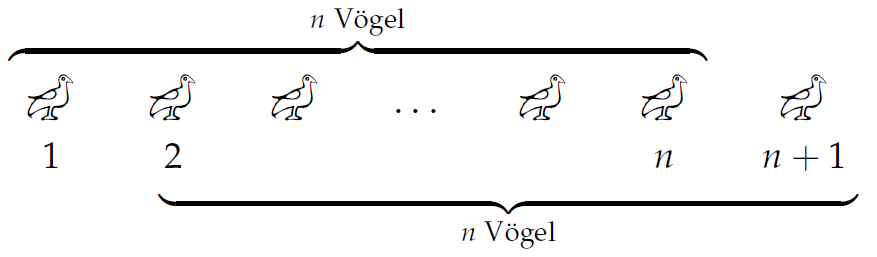
\includegraphics[scale=0.4]{induktion_voegel}
			\centering
		\end{figure}
	
		\only<5|handout:4>{
			Die Vögel $1, 2, ..., n$ bilden eine Menge mit genau $n$ Vögeln. Also haben sie nach IV alle die gleiche Farbe.\\ 
			Die Vögel $2, 3, ..., n + 1$ bilden auch eine Menge mit genau $n$ Vögeln. Also haben nach IV auch diese alle die gleiche Farbe.\\
			Damit haben auch die Vögel $1$ und $n + 1$ die gleiche Farbe, also haben alle Vögel die gleiche Farbe. $\qed$
		}
	\end{block}
	}
\end{frame}

\begin{frame}[t]{Vogelfarben: Auflösung}
	\begin{block}{Was geht schief?}
		\begin{figure}
			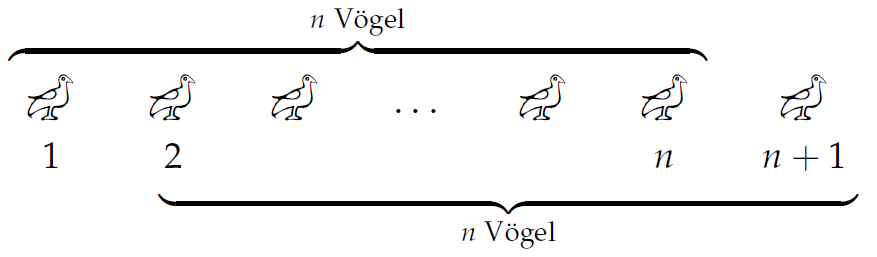
\includegraphics[scale=0.4]{induktion_voegel}
			\centering
		\end{figure}
		\pause
		Hübsches Bild. Scheint sauber. Ist bloß für $n=2$ völlig kaputt, die beiden Teilmengen \textbf{überlappen sich} dann nämlich \textbf{nicht}. \\
		\impl Wir können nicht sagen, dass der erste und letzte Vogel immer die gleiche Farbe haben. (Und wenn schon zwei Vögel nicht immer die gleiche Farbe haben, dann drei etc. auch nicht.) \\
		\impl Ganze Induktion \textbf{kaputt}. \frownie
	\end{block}	
	%Das Bild ist zwar außerordentlich hübsch, suggeriert aber leider etwas, was nicht immer stimmt: Für $n = 2$ überlappen sich die Teilmengen „ohne den ersten“ und „ohne den letzten“ Vogel nicht. Es ist also nicht erzwungen, dass beide Vögel die gleiche Farbe haben. (Und das macht „alles weitere“ auch kaputt: Wenn nicht immer 2 Vögel die gleiche Farbe haben, dann auch nicht immer 3 Vögel, usw.)
\end{frame}

% Induktion Übung

\begin{frame}{Und jetzt ihr}
    Betrachten Sie die Abbildung $f: \N_0 \to \N_0$, die wie folgt festgelegt ist:
    \begin{align*}
        f(0) = 0&&\forall n \in \N_0: f(n+1) = 2f(n) + n + 5
    \end{align*}
% 	Behauptung: \[\forall n \in \N_+ : \sum_{k=0}^{n}{\frac{1}{2^k}} = 2 \* \tuple{1 - \frac{1}{2^{n+1}}}\]
    Beweisen Sie durch vollständige Induktion, dass für jedes $n \in \N_0$ gilt:
    \[f(n) = 6(2^n - 1) - n\]
	\pause
	\begin{block}{Induktionsanfang}
		$n = 0$: $f(0)=0 = 6 \cdot 0 - 0 = 6 \cdot (2^0 - 1) - 0 $. \; \textbf{\checked}
	\end{block}
	\pause
	\begin{block}{Induktionsvoraussetzung}
		Für ein $n \in \N_0$ gelte: $f(n) = 6(2^n - 1) - n$.
	\end{block}
\end{frame}

\begin{frame}[t]
	\begin{block}{Induktionsvoraussetzung}
		Für ein $n \in \N_0$ gelte: $f(n) = 6(2^n - 1) - n$.
	\end{block}
	\uncover<+->{}
	\begin{block}{Induktionsschritt}
		Zeige die Aussage für $n+1$:\\
		\begin{align*}
			f(n+1)
				&= \uncover<+->{2f(n)+n+5}\\
				\uncover<+->{&\stackrel{\text{IV}}{=} 2(6(2^n-1)-n)+n+5\\}
				\uncover<+->{
				&= 6(2^{n+1}-2)-2n+n+5\\}
				\uncover<+->{
				&= 6(2^{n+1}-1)-6-n-1+6\\}
				\uncover<+->{
				&= 6(2^{n+1}-1)-(n+1) \qed}
		\end{align*}
	\end{block}
\end{frame}

\begin{frame}{Und jetzt ihr}
	Behauptung: \[\forall n \in \N_+ : \sum_{k=0}^{n}{\frac{1}{2^k}} = 2 \* \tuple{1 - \frac{1}{2^{n+1}}}\]
	\pause
	\begin{block}{Induktionsanfang}
		$n = 1$: $\sum_{k=0}^{1}{\frac{1}{2^k}} = \frac{3}{2} = 2 \* \frac{3}{4}$. \; \textbf{\checked}
	\end{block}
	\pause
	\begin{block}{Induktionsvoraussetzung}
		Für ein $n \in \N_0$ gelte: $\sum_{k=0}^{n}{\frac{1}{2^k}} = 2 \* \tuple{1 - \frac{1}{2^{n+1}}}$.
	\end{block}
\end{frame}

\begin{frame}[t]
	\uncover<+->{}
	\begin{block}{Induktionsschritt}
		Zeige die Aussage für $n+1$:\\
		\begin{align*}
			\sum_{k=0}^{n+1}{\frac{1}{2^k}}
				&= \uncover<+->{\underbrace{\sum_{k=0}^{n}{\frac{1}{2^k}}}_{\stackrel{\text{IV}}{=} 2 \* \tuple{1 - \frac{1}{2^{n+1}}}} + \frac{1}{2^{n+1}}}\\
				\uncover<+->{&= 2 \* \left(1 - \frac{1}{2^{n+1}}\right) + \frac{1}{2^{n+1}}\\
				&= 2 \* \left(1 - \frac{2}{2^{n+2}} + \frac{1}{2^{n+2}}\right)\\
				&= 2 \* \left(1 - \frac{1}{2^{(n+1)+1}}\right). \qed}
		\end{align*}
	\end{block}
\end{frame}

% Induktion Wörter Länge
% \begin{frame}{Und jetzt mit Wörtern}
% 	\begin{block}{Behauptung}
% 		Seien $A, B$ zwei beliebige Alphabete. Definiere die Funktion $f \from A^* \functionto A^*$,
% 		\begin{align*}
% 			f(\eps) &:= \eps \\
% 			\text{Für } w \in A^*, \mu \in A: \quad f(\mu \* w) &:= 
% 			\begin{cases}
% 				\mu \* f(w), &\mu \in B \\
% 				f(w), &\text{sonst}
% 			\end{cases}\\
% 		\end{align*}
	
% 	Dann gilt $\forall w \in A^*: \size{f(w)} \le \size w$.
% 	\end{block}
% \end{frame}

% \begin{frame}{Und jetzt mit Wörtern}
% 	Induktion über die Wortlänge ($n = \size w$):\\[0.5em]
% 	\pause
% 	\begin{block}{Induktionsanfang}
% 		$n = 0$: Nur das leere Wort hat Länge 0. Also $w = \eps$.\\
% 		$f(\eps) = \eps \impl \size{f(w)} = \size w = 0$. \; \textbf{\checked}
% 	\end{block}
% 	\pause
% 	\begin{block}{Induktionsvoraussetzung}
% 		Für \textbf{ein} $n \in \N_0$ gelte: Für alle Wörter der Länge $n$ über $A$ (also $w \in A^n$) ist $\size{f(w)} \le \size w$.
% 	\end{block}
% \end{frame}

% \begin{frame}{Und jetzt mit Wörtern}
% 	\begin{block}{Induktionsschritt}
% 		Zeige die Aussage für $n+1$:\\
% 		Sei $w \in A^{n+1}$ ein Wort der Länge $n+1$.\\
% 		\pause
% 		Dann teilen wir es auf in $w = \mu \* v$, wobei $\mu \in A$ und $v \in A^n$.\\
% 		Nach IV gilt: $\size{f(v)} \le \size v$.\\
% 		\pause
% 		\smallskip
% 		\textbf{Fall 1}: \\
% 			\quad $\mu \in B$: $f(w) = \mu \* f(v)$ \\
% 			\quad \impl $\size{f(w)} = 1 + \size{f(v)} \le 1 + \size v = 1+n = \size w$.\\
% 		\pause
% 		\smallskip
% 		\textbf{Fall 2}: \\
% 			\quad $\mu \notin B$: $f(w) = f(v)$ \\
% 			\quad \impl $\size{f(w)} = \size{f(v)} \le \size v = n \le n+1 = \size w$.\\
% 		\pause
% 		\smallskip
% 		Also gilt: $\size{f(w)} \le \size w. \qed$
% 	\end{block}
% \end{frame}